% This must be in the first 5 lines to tell arXiv to use pdfLaTeX, which is strongly recommended.
\pdfoutput=1
% In particular, the hyperref package requires pdfLaTeX in order to break URLs across lines.

\documentclass[11pt]{article}

% Remove the "review" option to generate the final version.
\usepackage[]{acl}

% Standard package includes
\usepackage{times}
\usepackage{latexsym}
\usepackage{booktabs}

%graphics package
\usepackage{graphicx}
\graphicspath{ {./figures/} }

% For proper rendering and hyphenation of words containing Latin characters (including in bib files)
\usepackage[T1]{fontenc}
% For Vietnamese characters
% \usepackage[T5]{fontenc}
% See https://www.latex-project.org/help/documentation/encguide.pdf for other character sets

% This assumes your files are encoded as UTF8
\usepackage[utf8]{inputenc}

% This is not strictly necessary, and may be commented out,
% but it will improve the layout of the manuscript,
% and will typically save some space.
\usepackage{microtype}

% If the title and author information does not fit in the area allocated, uncomment the following
%
%\setlength\titlebox{<dim>}
%
% and set <dim> to something 5cm or larger.

\title{HEVS-TUW at SemEval-2023 Task 8}

% Author information can be set in various styles:
% For several authors from the same institution:
% \author{Author 1 \and ... \and Author n \\
%         Address line \\ ... \\ Address line}
% if the names do not fit well on one line use
%         Author 1 \\ {\bf Author 2} \\ ... \\ {\bf Author n} \\
% For authors from different institutions:
% \author{Author 1 \\ Address line \\  ... \\ Address line
%         \And  ... \And
%         Author n \\ Address line \\ ... \\ Address line}
% To start a seperate ``row'' of authors use \AND, as in
% \author{Author 1 \\ Address line \\  ... \\ Address line
%         \AND
%         Author 2 \\ Address line \\ ... \\ Address line \And
%         Author 3 \\ Address line \\ ... \\ Address line}


\author{Anjani Dhrangadhariya\hspace{1pt}$^{{{\bf 1,2}}\dag}$ \hspace{.7cm} Wojciech Kusa\hspace{1pt}$^{{\bf 3}\dag}$ \\[0.15cm] {\bf Henning Müller\hspace{1pt}$^{{\bf 1,2}}$}  \hspace{.7cm}  {\bf Allan Hanbury\hspace{1pt}$^{{\bf 3}}$}
\\[0.4cm]
{$^1$University of Geneva, Geneva, Switzerland} \\
{$^2$HES-SO Valais-Wallis, Sierre, Switzerland} \\
{\tt \{anjani.dhrangadhariya,henning.mueller\}@hevs.ch} \\
{$^2$TU Wien, Vienna, Austria} \\
{\tt \{wojciech.kusa,allan.hanbury\}@tuwien.ac.at} \\
}


\begin{document}
\maketitle
{\let\thefootnote\relax\footnotetext{$\dag$ Equal contribution.}}

\begin{abstract}
This paper describes HEVS-TUW team submission to the SemEval-2023 Task 8: Causal Claims.
We participated in two subtasks: (1):causal claims detection and (2): PIO identification.
For task 1, we experimented with an ensemble of weakly supervised question detection and fine-tuned Transformer NER models.
For task 2 ...
Our results for Subtask 1 show moderate benefit from ensembling models pretrained on independent categories.

\end{abstract}

\section{Introduction}

% 
Identification and verification of causal claims from unstructured text data is an important task for various decision-making processes, particularly in the field of healthcare. The SemEval-2023 Task 8~\cite{CausalClaims} aims to advance the state-of-the-art in this area by focusing on two subtasks: identification of causal claims and extraction of Population, Intervention, and Outcome (PIO) entities.

% 
The first subtask involves identifying the span of text that contains one of the four entities: a \emph{causal claim}, a \emph{personal experience}, a \emph{personal experience based on a claim} or a \emph{question}. 
This can be done at sentence level, but it is possible that only a part of a sentence is annotated with one of these categories. 
The second subtask involves extracting the PIO frame related to the identified causal claim in a text snippet using an end-to-end deep learning model.
The model utilizes both word-level, including contextual information and character-level features capturing different aspects of the data.

Our approach to subtask one fared well at rank 4, with F1 a 32.77\% better than the last ranked approach and 12.7\% behind the approach ranked 1.
For subtask 2, the approach ranks second last on the leaderboard, and the system mainly struggles with identifying the population frame.
These subtasks have potential applications in content moderation, insurance claim identification, and hypothesis generation from clinical notes.
We believe that the shared task will motivate further research in this direction and lead to the development of more effective and accurate methods for causal claim identification and PIO frame extraction.
%
%
%
\section{Background}
\label{background}
%
The task of identifying causal claims and extracting the associated PIO frame from unstructured text data has received increasing attention in recent years.
This is particularly relevant in the healthcare domain, where large amounts of medical notes, research articles, and patient forums are generated on a daily basis.
Manual extraction of causal claims and PIO frames from such data is a time-consuming and error-prone process. Therefore, there is a growing interest in developing automated methods that can identify and extract such information with high accuracy.

While these methods have shown promising results, there is still room for improvement in terms of accuracy and efficiency.
The SemEval-2023 Task 8 provides an opportunity for researchers to develop novel methods for causal claim identification and PIO frame extraction and to benchmark their performance against state-of-the-art methods.
We hope that the shared task will lead to the development of more effective and accurate methods for identifying and extracting causal claims and PIO frames from unstructured text data.

%Anjani: Background for the PIO extraction task
For a decade, PIO extraction was limited to sentence-level information extraction due to the unavailability of frame-annotated datasets.~\cite{boudin2010combining,jin2018pico}
After the release of the EBM-PICO corpus, the extraction efforts moved to span and frame extraction.~\cite{nye2018corpus}
Nonetheless, previous studies on PIO frame extraction primarily concentrated on extracting them from well-written, peer-reviewed literature.~\cite{brockmeier2019improving,zhang2020unlocking,dhrangadhariya2021end}
The SemEval-2023 task 8 overtakes the challenge of extracting these frames from noisy social media data.
The task organizers provide 597, English-language PIO labelled Reddit posts.
We approach PIO frame extraction as sequence labelling and use a combination of deep learning and rule-based approach that captures multiple feature representations from the data, as the dataset is relatively small.
%
%
%
\section{System overview}
\label{system_over}
%
We participated in both subtasks of SemEval-2023 Task 8. 
In this section we describe our approach.
%
%
%
\subsection{Subtask 1} \label{sec:system1}
\label{subsec:syst_task1}
%
For Subtask 1 we implement two components: weakly supervised question detection and a Transformers-based fully supervised entity recogniton.
We treat the task 1 as a named entity recognition task.

\subsubsection*{Question detector}


We design a weakly supervised question detector approach (QD).
We use a spaCy sentencizer to split the text into sentences.
Next we search for the occurrences of the question mark token `?'. 


% 2. weakly questions: st1\_test\_predictions.csv (different folder)

\subsubsection*{Supervised NER}


We fine-tune five models using training subset of the released trainset:

\begin{enumerate}
\item RoBERTa$_A$ -- RoBERTa model~\cite{Liu2019RoBERTaAR} trained on all entities. % //newstorage5/wkusa/models/pico/ph1-all/roberta/final-model.pt trained for 25 epochs: st1\_test\_flair\_roberta.csv
\item distilBERT$_A$ -- distilBERT model~\cite{Sanh2019DistilBERTAD} trained on all entities.  %all: all\_flair\_submission.csv
\item  distilBERT$_q$ --  distilBERT trained on extracting only questions. %$_q$distil question  question\_flair\_submission.csv
\item distilBERT$_{pe}$ -- distilBERT model trained on personal experience entities %: st1\_test\_flair\_per\_exp.csv
\item distilBERT$_c$ -- distilBERT model trained on claim entities %: st1\_test\_flair\_per\_exp.csv
\end{enumerate}

The three last models are trained 



%
%
%
\subsection{Subtask 2}
\label{system:task2}
%
PIO extraction was a three-part system: a text preprocessing module, a deep learning entity extraction pipeline and a rule-based approach to combine separate PIO predictions.
%
%
%
\subsubsection{Preprocessing module}
%
The PIO dataset was processed to parse annotation from the Reddit posts.
The empty or partially deleted samples were removed leaving 522 samples.
Next, the text tokens were enriched with the part-of-the-speech (POS) tags and token lemmas using spaCy~\footnote{https://spacy.io/}.
%
%
%
\subsubsection{Deep learning module}
%
%
%
The deep learning system was built on combining the feature extractors (word-level and character-level) followed by a learning component.
%
\paragraph{Word-level features: }
%
The word-level features included transformer and POS inputs.
Transformer models, specifically \textbf{RoBERTa} and \textbf{BioMed-RoBERTa}, were used to extract $\mathbf{T}^{d \times l}$ dimensional contextual features from input samples, where l is maximum input length for transformers.~\cite{liu2019roberta,gururangan2020don}
POS information help NLP models better understand the syntactic structure of a sentence.
The token POS tags were encoded into $\mathbf{P}^{d \times l}$ dimensional one-hot sparse \textbf{POS} embeddings.
%The \textbf{POS} embeddings were one-hot sparse vectors 30-dimensional vectors comprising POS tags generated by spaCy. 
POS features were either \textbf{one-hot} encoded or transformed using a \textbf{BiLSTM} (bidirectional Long short-term memory) to encode long-term dependencies and learn a task-specific grammatical structure from the input samples.~\cite{hochreiter1997long}
Transformer and POS features were concatenated to obtain a word-level representation.
%Anjani: Include a figure with character and word representations
\begin{figure}[!htbp]
    \centering
    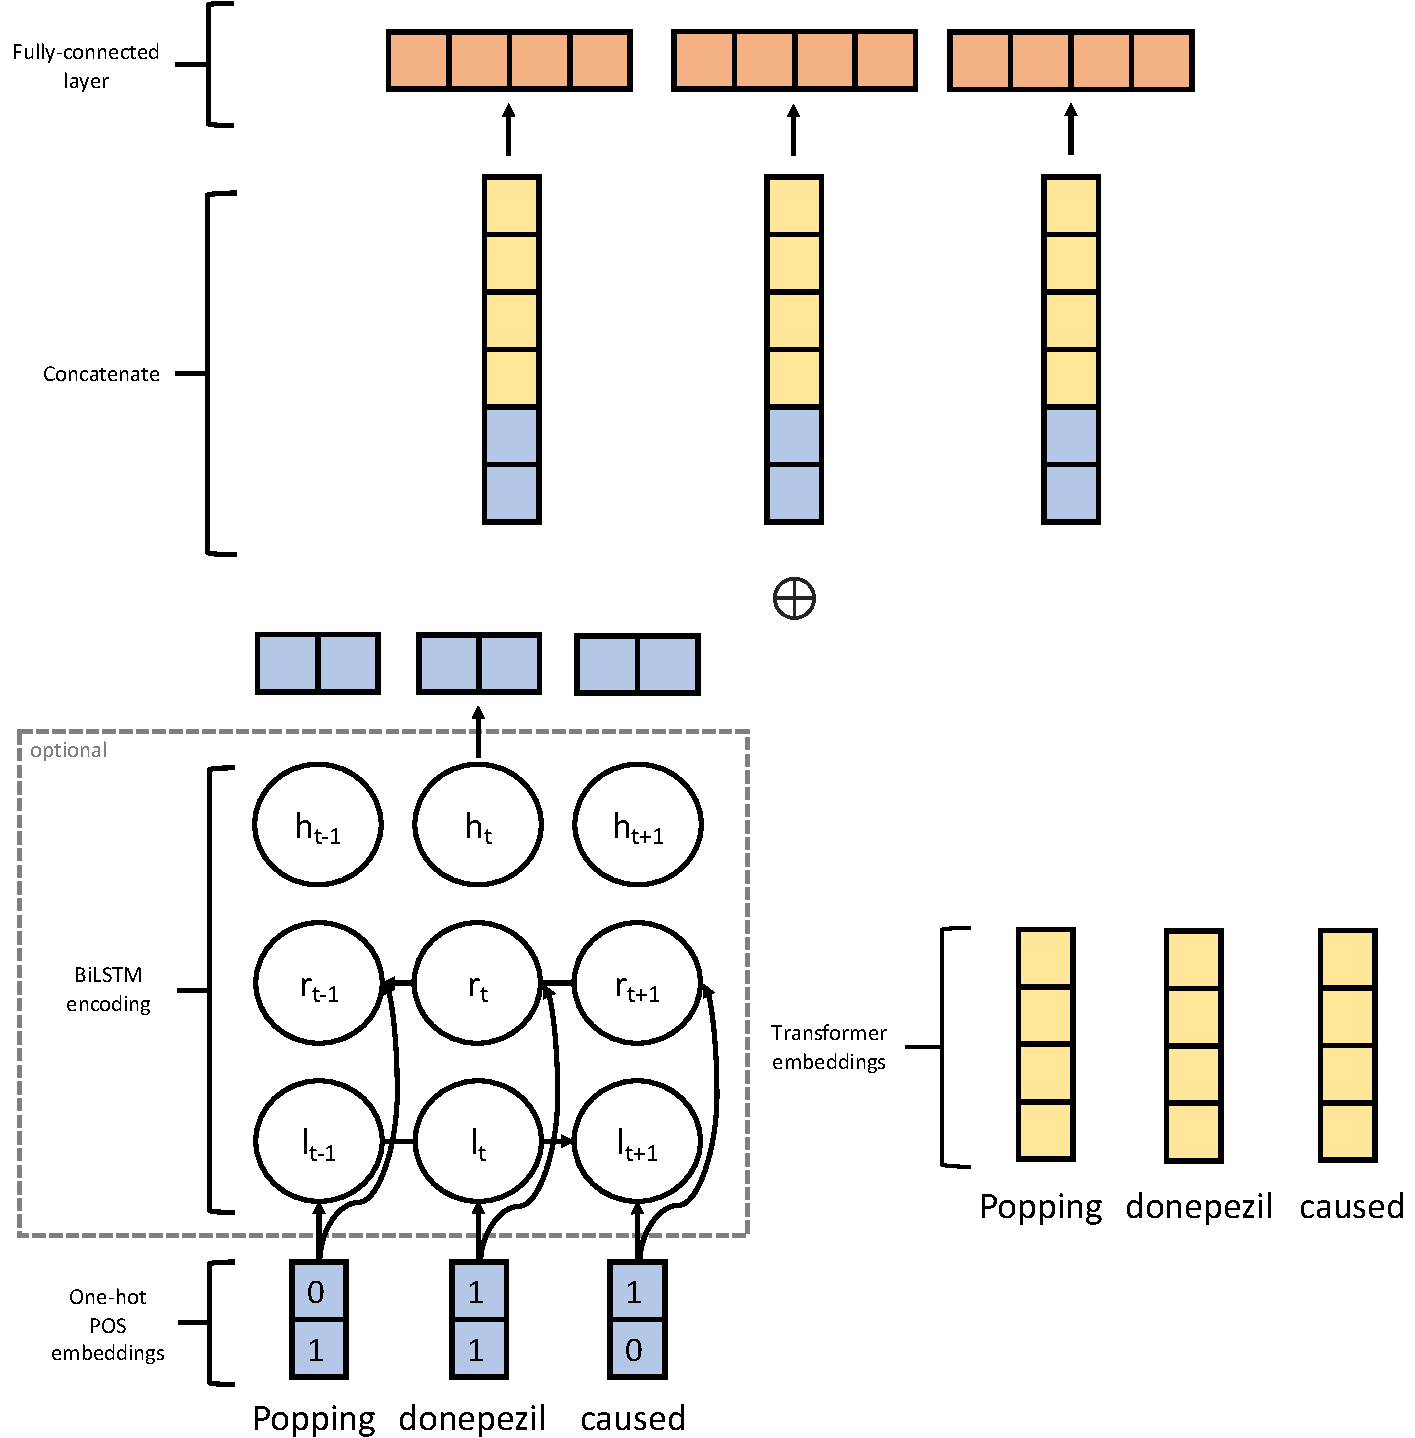
\includegraphics[width=\columnwidth]{figures/word_arch.pdf}
    \caption{Word representation using concatenation of the POS embeddings (with or without BiLSTM transformation) and transformer embeddings (yellow).}
    \label{fig:task2_word}
\end{figure}
%
%
%
\paragraph{Character-level features: } 
%
\textbf{Orthographic features} are the character-based features that encapsulate capitalization, punctuation, word shape, and other orthographic features; e.g., "SemEval 2023!" encoded as "CccCccc nnnnp". 
\textbf{Character features} are sparser matrices encapsulating character-level information, including alphabet and individual punctuation.
The characters are embedded into a $\mathbf{C}^{d \times wl}$ dimensional space, where d is the dimension of the features per character and $wl$ is the maximum length of characters per word.
%An orthographic token encoding was six-dimensional, and character encoding was 28-dimensional, with a maximum token length of 20 characters applying post-padding on shorter words and truncating the longer ones.
Our system used either the orthographic or the character features which were transformed using a 1-dimensional convolutional neural network (\textbf{1D-CNN}) followed by either a max pooling (\textbf{MP}) or global average pooling (\textbf{GAP}) operation.~\cite{zhou2016learning}
Next, the results are fed through a fully-connected layer via ReLU (Rectified Linear Unit) to obtain a character-level representation.
Both the word-level features and CNN-transformed character features were concatenated and fed to a \textbf{linear layer} to predict the entity sequence.
%
\begin{figure}[!htbp]
    \centering
    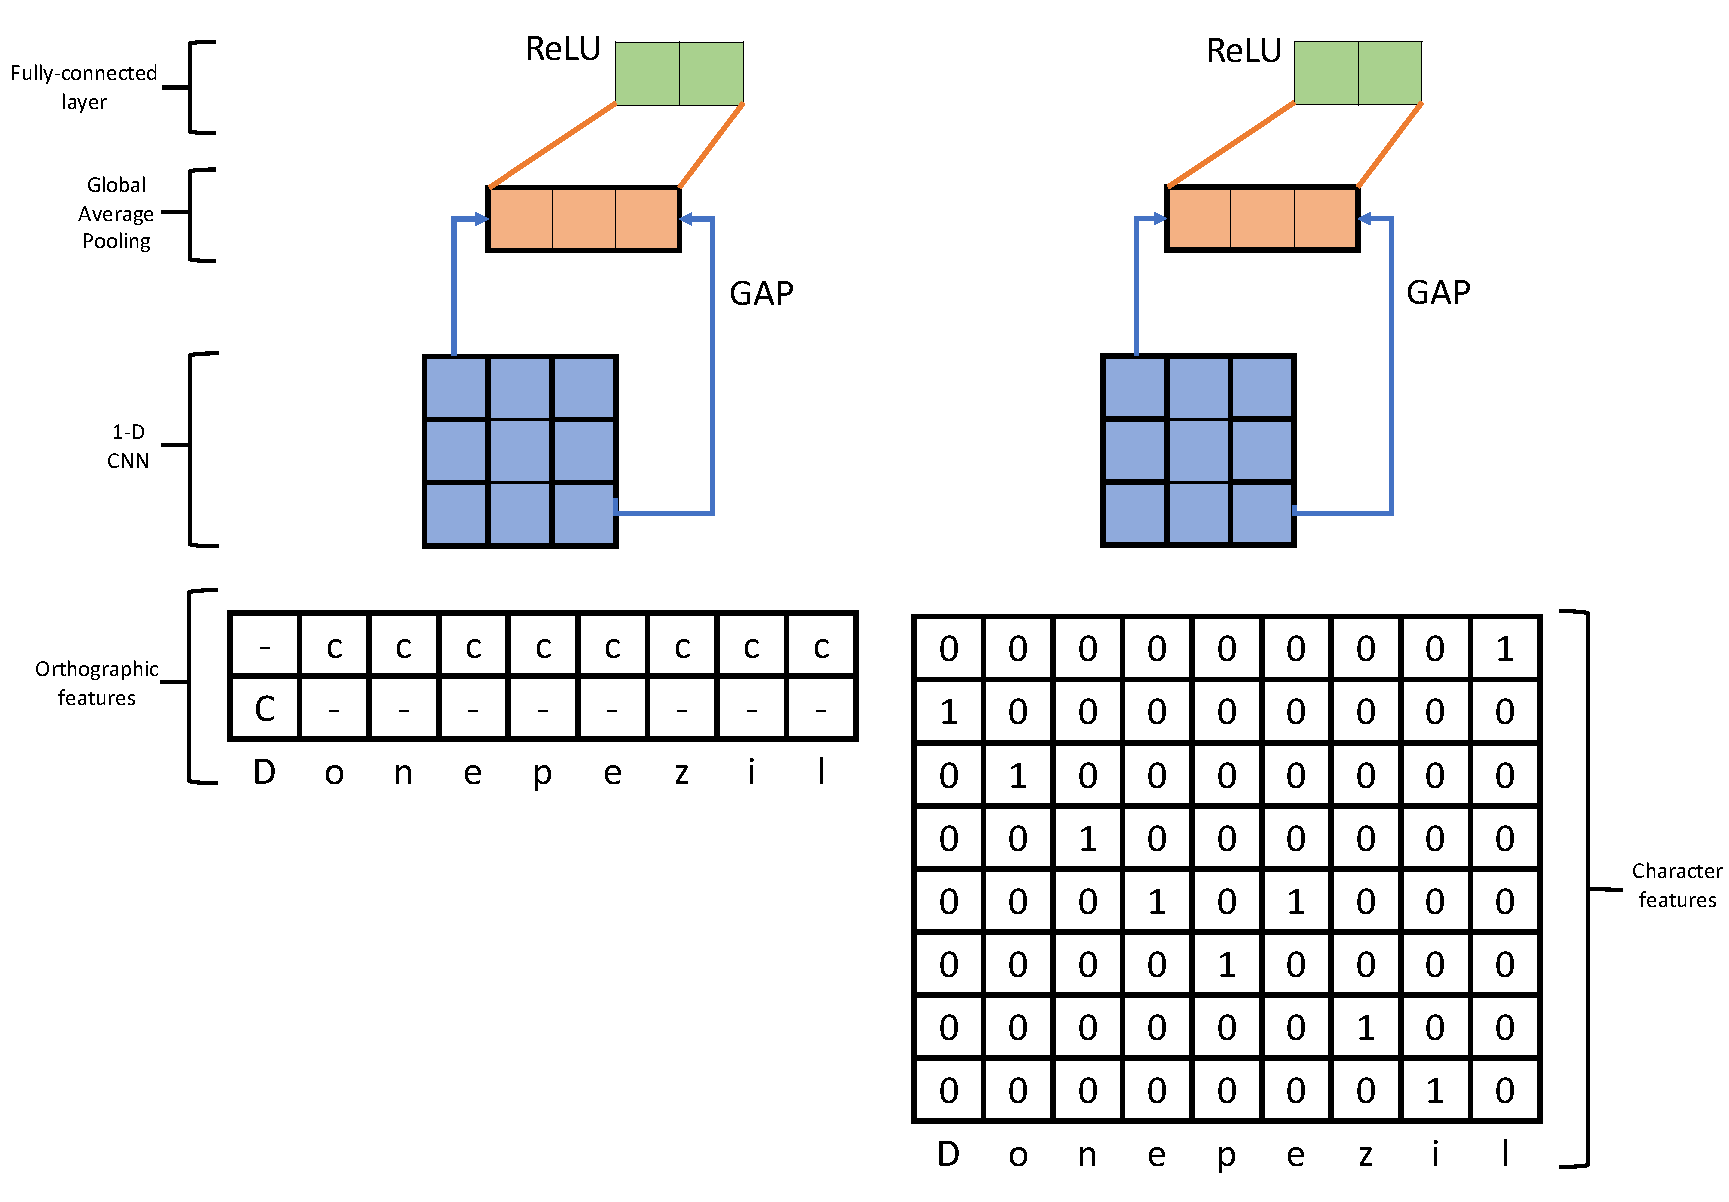
\includegraphics[width=\columnwidth]{figures/word_arch2.pdf}
    \caption{Character representation.}
    \label{fig:task2_char}
\end{figure}
%
%
%
\section{Experimental setup}
In this section we describe our experimental setup for subtasks (1) and (2). 
%
%
%
% How data splits (train/dev/test) are used.
% Key details about preprocessing, hyperparameter tuning, etc. that a reader would need to know to replicate your experiments. If space is limited, some of the details can go in an Appendix.
% External tools/libraries used, preferably with version number and URL in a footnote.
% Summarize the evaluation measures used in the task.
% You do not need to devote much—if any—space to discussing the organization of your code or file formats.
Runs for both the subtasks are evaluated using macro F1-score measure.
%
%
%
\subsection{Subtask 1}

We train all transformer based models for 30 epochs. 
Following task organisers, we perform splitting on whitespaces.
We use 80\% of training data for training models and 20\% for validation.
We use Flair to implement our NER models~\cite{Akbik2019FLAIRAE}.

For subtask 1 we submit four runs which are ensembles of models described in Section \ref{sec:system1}:

\begin{itemize}
\item \textbf{Run 1} - QD + distilBERT$_q$ + distilbert$_A$
\item \textbf{Run 2} - QD + distilBERT$_q$ + distilBERT$_{pe}$ + distilBERT$_A$
\item \textbf{Run 3} - QD + distilBERT$_q$ + distilBERT$_{pe}$ + RoBERTa$_A$
\item \textbf{Run 4} - QD + distilBERT$_q$ + distilBERT$_{pe}$ + distilBERT$_A$ + RoBERTa$_A$ 
\end{itemize}

Run 4 is like Run 2 just adds roberta.
Run 3 is like Run 2 but last model is switched.
We do the majority voting for non-null predictions, i.e. whenever at least one model predicts some entity we 

%Runs are evaluated using macro F1-score measure. %Anjani: moved this sentence above as macro F1 was used for both the subtasks and was redundant. 
%
%
%
\subsection{Subtask 2}
\label{exps:task2}
%
For subtask 2, we submitted four runs, each an ensemble for PIO classes, and with the following architecture whose components are described in Section \ref{system:task2}.
Three separate training experiments were carried out for each PIO class.
Each experiment was averaged over the three most common random seeds in python, 0,1 and 42.
Individual PIO predictions were combined based on majority voting with a random tie break.
The dataset was divided into a training (80\%) and test sets (20\%).
%
\begin{enumerate}
    \item Run 1: RoBERTa embeddings were concatenated to BiLSTM transformed POS embeddings. Character-level orthographic embeddings were CNN transformed and fed to a fully connected layer followed by average pooling. Processed word and character representations were fed to a linear layer to predict the PIO entity.
    \item Run 2: RoBERTa embeddings were concatenated to one-hot encoded POS embeddings. Character embeddings were CNN transformed and fed to a fully connected layer followed by average pooling. Processed word and character representations were fed to a linear layer to predict the PIO entity.
    \item Run 3: RoBERTa embeddings were concatenated to one-hot encoded POS embeddings. Character-level orthographic embeddings were CNN transformed and fed to a fully connected layer followed by GAP. Processed word and character representations were fed to a linear layer to predict the PIO entity.
    \item Run 4: RoBERTa embeddings were concatenated to BiLSTM transformed POS embeddings. Character-level orthographic embeddings were CNN transformed and fed to a fully connected layer followed by GAP. Processed word and character representations were fed to a linear layer to predict the PIO entity.
    \item Run 5: Three different architectures, each corresponding to PIO classes, were used for the fifth run. Ensemble 14 (P), 13 (I) BRoB, 1 (O)   
\end{enumerate}
%
%
%
\section{Results}

\subsection{Subtask 1}

Results for our submissions in Subtask 1 are presented in Table \ref{tab:task_1}. Our approach based on adding distilbert with personal experience improves recall for these entities.

\begin{table}[ht]
    \centering
    \begin{tabular}{lccc}
        \toprule
        Run & Precision & Recall & F1-score \\
        \midrule
        Run 1 & 68.13 & 61.21 & 64.48 \\
        Run 2 & 66.81 & 66.12 & 66.46 \\
        Run 3 & 70.32 & 63.38 & 64.52 \\
        Run 4 & 68.73 & 62.90 & 65.70 \\
        \bottomrule
    \end{tabular}
    \caption{Results from Subtask 1.}
    \label{tab:task_1}
\end{table}
%
%
%
\subsection{Subtask 2}
\label{res:task2}
%
F1-scores for the official SemEval-2023 test set for the subtask 2 are presented in Table \ref{tab:task_2}.

%
\begin{table}[ht]
    \centering
    \begin{tabular}{lccc}
        \toprule
          & \multicolumn{3}{c}{Macro F1} \\
         \hline
        Run & Population & Intervention & Outcome \\
        \midrule
        Run 1 & 12.39 & 19.43 & 22.10 \\
        Run 2 & 21.30 & 20.05 & 20.33 \\
        Run 3 & 17.44 & 26.39 & 22.78 \\
        Run 4 & 11.54 & 25.63 & 22.74 \\
        Run 5 & 08.18 & 16.47 & 12.28 \\
        \bottomrule
    \end{tabular}
    \caption{Subtask 2 results: F1-score on the official SemEval-2023 test set for the Population, Intervention and Outcome classes over five runs.}
    \label{tab:task_2}
\end{table}


\section{Conclusion}


% These instructions are for authors submitting papers to *ACL conferences using \LaTeX. They are not self-contained. All authors must follow the general instructions for *ACL proceedings,\footnote{\url{http://acl-org.github.io/ACLPUB/formatting.html}} and this document contains additional instructions for the \LaTeX{} style files.

% The templates include the \LaTeX{} source of this document (\texttt{acl.tex}),
% the \LaTeX{} style file used to format it (\texttt{acl.sty}),
% an ACL bibliography style (\texttt{acl\_natbib.bst}),
% an example bibliography (\texttt{custom.bib}),
% and the bibliography for the ACL Anthology (\texttt{anthology.bib}).

% \section{Engines}

% To produce a PDF file, pdf\LaTeX{} is strongly recommended (over original \LaTeX{} plus dvips+ps2pdf or dvipdf). Xe\LaTeX{} also produces PDF files, and is especially suitable for text in non-Latin scripts.

% \section{Preamble}

% The first line of the file must be
% \begin{quote}
% \begin{verbatim}
% \documentclass[11pt]{article}
% \end{verbatim}
% \end{quote}

% To load the style file in the review version:
% \begin{quote}
% \begin{verbatim}
% \usepackage[review]{acl}
% \end{verbatim}
% \end{quote}
% For the final version, omit the \verb|review| option:
% \begin{quote}
% \begin{verbatim}
% \usepackage{acl}
% \end{verbatim}
% \end{quote}

% To use Times Roman, put the following in the preamble:
% \begin{quote}
% \begin{verbatim}
% \usepackage{times}
% \end{verbatim}
% \end{quote}
% (Alternatives like txfonts or newtx are also acceptable.)

% Please see the \LaTeX{} source of this document for comments on other packages that may be useful.

% Set the title and author using \verb|\title| and \verb|\author|. Within the author list, format multiple authors using \verb|\and| and \verb|\And| and \verb|\AND|; please see the \LaTeX{} source for examples.

% By default, the box containing the title and author names is set to the minimum of 5 cm. If you need more space, include the following in the preamble:
% \begin{quote}
% \begin{verbatim}
% \setlength\titlebox{<dim>}
% \end{verbatim}
% \end{quote}
% where \verb|<dim>| is replaced with a length. Do not set this length smaller than 5 cm.

% \section{Document Body}

% \subsection{Footnotes}

% Footnotes are inserted with the \verb|\footnote| command.\footnote{This is a footnote.}

% \subsection{Tables and figures}

% See Table~\ref{tab:accents} for an example of a table and its caption.
% \textbf{Do not override the default caption sizes.}

% \begin{table}
% \centering
% \begin{tabular}{lc}
% \hline
% \textbf{Command} & \textbf{Output}\\
% \hline
% \verb|{\"a}| & {\"a} \\
% \verb|{\^e}| & {\^e} \\
% \verb|{\`i}| & {\`i} \\ 
% \verb|{\.I}| & {\.I} \\ 
% \verb|{\o}| & {\o} \\
% \verb|{\'u}| & {\'u}  \\ 
% \verb|{\aa}| & {\aa}  \\\hline
% \end{tabular}
% \begin{tabular}{lc}
% \hline
% \textbf{Command} & \textbf{Output}\\
% \hline
% \verb|{\c c}| & {\c c} \\ 
% \verb|{\u g}| & {\u g} \\ 
% \verb|{\l}| & {\l} \\ 
% \verb|{\~n}| & {\~n} \\ 
% \verb|{\H o}| & {\H o} \\ 
% \verb|{\v r}| & {\v r} \\ 
% \verb|{\ss}| & {\ss} \\
% \hline
% \end{tabular}
% \caption{Example commands for accented characters, to be used in, \emph{e.g.}, Bib\TeX{} entries.}
% \label{tab:accents}
% \end{table}

% \subsection{Hyperlinks}

% Users of older versions of \LaTeX{} may encounter the following error during compilation: 
% \begin{quote}
% \tt\verb|\pdfendlink| ended up in different nesting level than \verb|\pdfstartlink|.
% \end{quote}
% This happens when pdf\LaTeX{} is used and a citation splits across a page boundary. The best way to fix this is to upgrade \LaTeX{} to 2018-12-01 or later.

% \subsection{Citations}

% \begin{table*}
% \centering
% \begin{tabular}{lll}
% \hline
% \textbf{Output} & \textbf{natbib command} & \textbf{Old ACL-style command}\\
% \hline
% \citep{Gusfield:97} & \verb|\citep| & \verb|\cite| \\
% \citealp{Gusfield:97} & \verb|\citealp| & no equivalent \\
% \citet{Gusfield:97} & \verb|\citet| & \verb|\newcite| \\
% \citeyearpar{Gusfield:97} & \verb|\citeyearpar| & \verb|\shortcite| \\
% \hline
% \end{tabular}
% \caption{\label{citation-guide}
% Citation commands supported by the style file.
% The style is based on the natbib package and supports all natbib citation commands.
% It also supports commands defined in previous ACL style files for compatibility.
% }
% \end{table*}

% Table~\ref{citation-guide} shows the syntax supported by the style files.
% We encourage you to use the natbib styles.
% You can use the command \verb|\citet| (cite in text) to get ``author (year)'' citations, like this citation to a paper by \citet{Gusfield:97}.
% You can use the command \verb|\citep| (cite in parentheses) to get ``(author, year)'' citations \citep{Gusfield:97}.
% You can use the command \verb|\citealp| (alternative cite without parentheses) to get ``author, year'' citations, which is useful for using citations within parentheses (e.g. \citealp{Gusfield:97}).

% \subsection{References}

% \nocite{Ando2005,borschinger-johnson-2011-particle,andrew2007scalable,rasooli-tetrault-2015,goodman-etal-2016-noise,harper-2014-learning}

% The \LaTeX{} and Bib\TeX{} style files provided roughly follow the American Psychological Association format.
% If your own bib file is named \texttt{custom.bib}, then placing the following before any appendices in your \LaTeX{} file will generate the references section for you:
% \begin{quote}
% \begin{verbatim}
% \bibliographystyle{acl_natbib}
% \bibliography{custom}
% \end{verbatim}
% \end{quote}

% You can obtain the complete ACL Anthology as a Bib\TeX{} file from \url{https://aclweb.org/anthology/anthology.bib.gz}.
% To include both the Anthology and your own .bib file, use the following instead of the above.
% \begin{quote}
% \begin{verbatim}
% \bibliographystyle{acl_natbib}
% \bibliography{anthology,custom}
% \end{verbatim}
% \end{quote}

% Please see Section~\ref{sec:bibtex} for information on preparing Bib\TeX{} files.

% \subsection{Appendices}

% Use \verb|\appendix| before any appendix section to switch the section numbering over to letters. See Appendix~\ref{sec:appendix} for an example.

% \section{Bib\TeX{} Files}
% \label{sec:bibtex}

% Unicode cannot be used in Bib\TeX{} entries, and some ways of typing special characters can disrupt Bib\TeX's alphabetization. The recommended way of typing special characters is shown in Table~\ref{tab:accents}.

% Please ensure that Bib\TeX{} records contain DOIs or URLs when possible, and for all the ACL materials that you reference.
% Use the \verb|doi| field for DOIs and the \verb|url| field for URLs.
% If a Bib\TeX{} entry has a URL or DOI field, the paper title in the references section will appear as a hyperlink to the paper, using the hyperref \LaTeX{} package.

\section*{Acknowledgements}
\label{acknowledgements}
%
This work was supported by the EU Horizon 2020 ITN/ETN on Domain Specific Systems for Information Extraction and Retrieval -- DoSSIER (H2020-EU.1.3.1., ID: 860721) and HES-SO Valais-Wallis, Sierre, Switzerland.
%
%
%
% Entries for the entire Anthology, followed by custom entries
\bibliography{anthology,custom}
\bibliographystyle{acl_natbib}

% \appendix

% \section{Example Appendix}
% \label{sec:appendix}

% This is an appendix.

\end{document}
